\chapter{ZIC Partitioning}
This chapter describes the architectural partitioning of the major ZIC interfaces and components, and introduces the functionality of the major ZIC components, the Priority Resolver and Interrupt Request Generator. It contains the following sections:

\begin{itemize}
    \item \hyperref[sec:about-zix-partition]{About ZIC partitioning}
    \item \hyperref[sec:priority-resolve]{Priority Resolver}
    \item \hyperref[sec:interrupt-request-generate]{Interrupt Request Generator}
\end{itemize}
\newpage

\section{About ZIC partitioning}
\label{sec:about-zix-partition}
ZIC architecture consists of two functional blocks; a Priority Resolver and an Interrupt Request Generator. Therefore, as Figure \ref{fig:zic_partitioning} shows, the partitioning of the ZIC is as follows:

\vspace{1cm}
\begin{tabular}{p{6cm} p{8.25cm}}
    \textbf{\hyperref[sec:priority-resolve]{Priority Resolver}} &  The Priority Resolver block captures the external interrupts and decides which interrupt has the highest priority and is eligible to be sent to the core.\\
    \textbf{\hyperref[sec:interrupt-request-generate]{Interrupt Request Generator}} & The Interrupt Request Generator block takes the highest priority interrupt from the priority resolver and conditionally sends a request to the processor if the interrupt has sufficient priority.\\
    \textbf{\hyperref[subsec:zic-register-mem-map]{ZIC Memory-mapped registers}} & The ZIC Memory-mapped registers consists of registers for ZIC configuration, information and other book-keeping registers like interrupt-pending, acknowledgement, end-of-interrupt registers.   \\
    \textbf{\hyperref[subsec:zic-csrs-mem-map]{ZIC CSRs}} & ZIC CSRs are interrupt handling registers that are adopted from Basic Machine-mode CSRs with some changes and additional registers. \\
\end{tabular}
\vspace{0.5cm}

The ZIC interacts with the ZIC Memory-mapped register and the CSRs. The RISC-V core has access to ZIC's memory-mapped registers using load-store instruction and CSRs using CSR op-codes.

\vspace{1cm}
\begin{figure}[H]
    \centering
    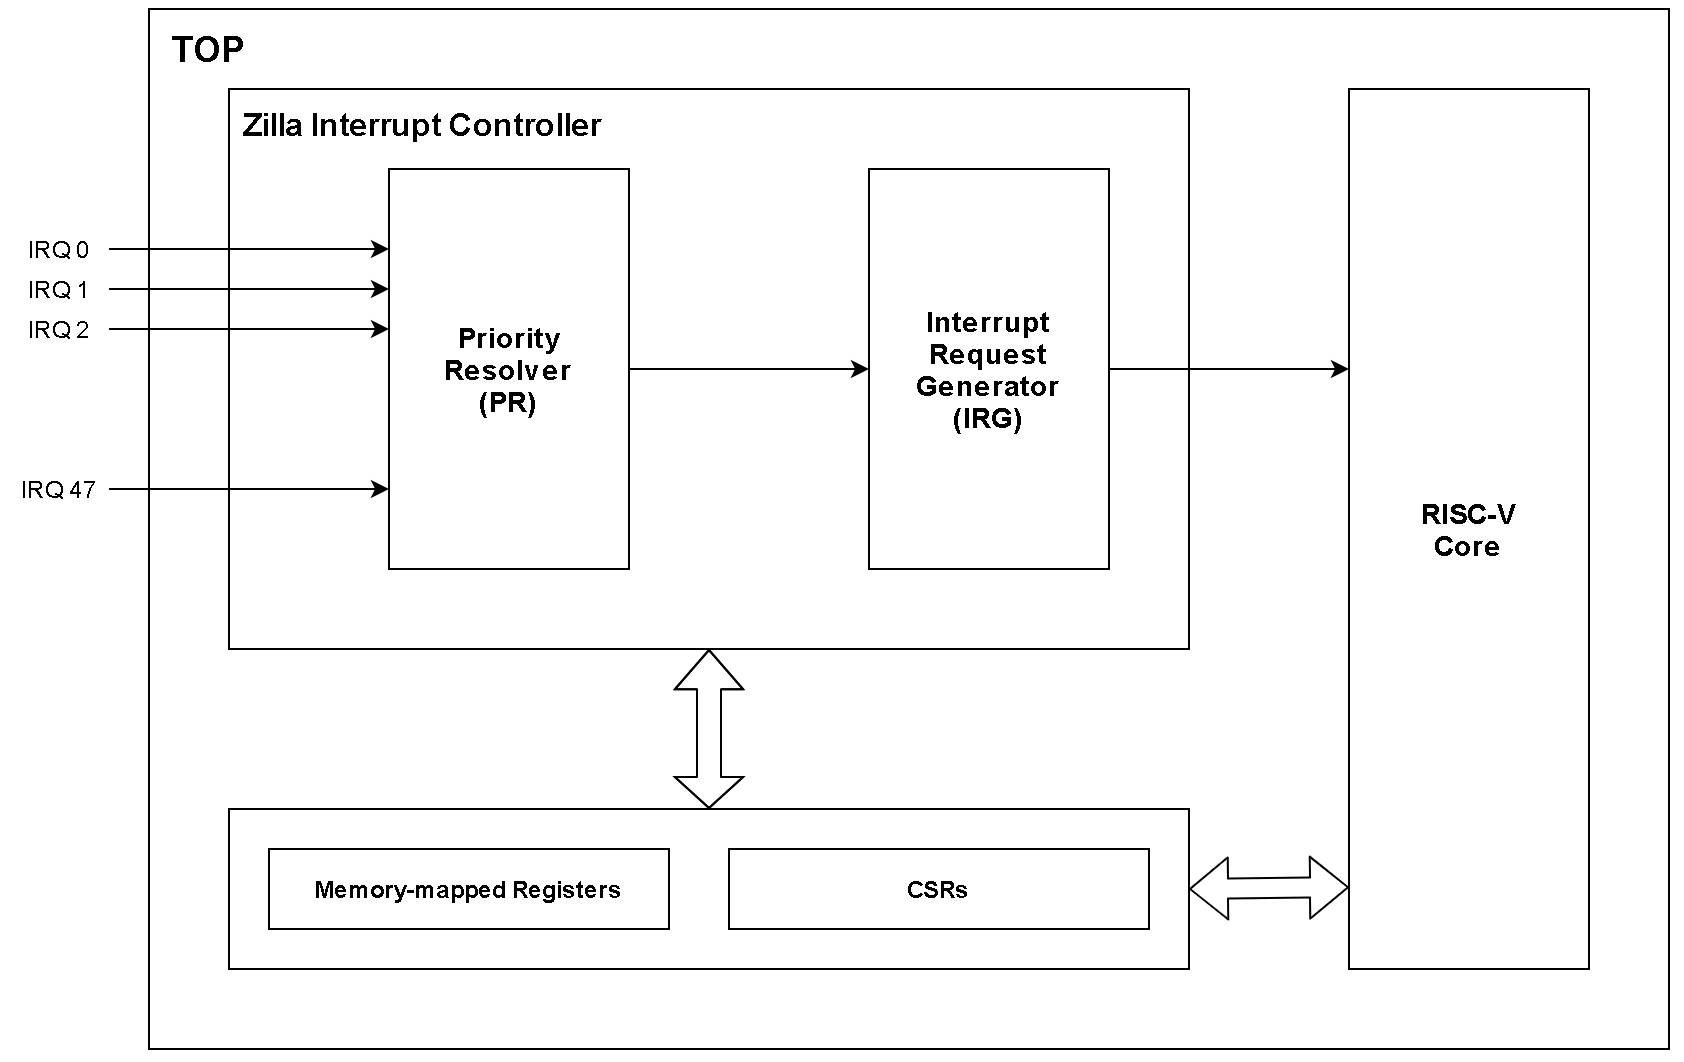
\includegraphics[width = 14cm]{images/ZIC.png}
    \vspace{1cm}
    \caption{\textbf{ZIC Partitioning}}
    \label{fig:zic_partitioning}
\end{figure}

\section{Priority Resolver}
\label{sec:priority-resolve}
The Priority Resolver block is responsible for  the following functionality.
\begin{enumerate}
    \item Provide an interface for all the external interrupts.
    \item Control the interrupt entry.
    \item Control the pending state of the interrupt.
    \item Assignment of level priority assignment for the pending interrupts and storing it in local buffers.
    \item Comparison of local buffers to obtain interrupt with highest level-priority value.
    \item Send the highest next pending interrupt to the Interrupt request generator.
\end{enumerate}

The Priority Resolver keeps track of new interrupts till the Interrupt Request Generator generates interrupt requests to the processor core. If any new interrupt is asserted from the source and has a higher level, the highest next pending register \texttt{zic\_nxtp\_int} is updated.

\subsection{Interrupt IDs}

\section{Interrupt Request Generator}
\label{sec:interrupt-request-generate}
The Interrupt Request Generator has the following functionality;
\begin{enumerate}
    \item Check for Sufficient Level-Priority.
    \item Update CSRs .
    \item Send a request to the core.
\end{enumerate}

This indicates the start of the interrupt service routine.

Once the processor completes the execution of the requested interrupt handler, it will write the corresponding ID into the end of the interrupt register \texttt{zi\_eoi}. Interrupt Request Generator detects this processor write and sends the new request for the next pending interrupt.
